%!TEX root = ../Bachelorarbeit.tex
\chapter{Anbindung externer Komponenten}
In diesem Kapitel wird zunächst der asynchrone Aufbau des Projektes näher erläutert. Im Anschluss daran wird die Anbindung von Erweiterungen an Project-Zoom betrachtet.

\section{Eventsystem}
Ein Eventsystem basiert auf dem Prinzip des Abonnierens und Veröffentlichens von Nachrichten und modelliert eine Eine-zu-Viele-Relation. Ein sogenannter \tete{Publisher} sendet seine Events, welche anschließend vom \tete{Dispatcher} an die \tete{Subscriber} verteilt werden. Die Subscriber können dieses Event schließlich abarbeiten. Dabei entsteht eine Asynchronität, da der Sender beim Emittieren einer Nachricht sofort sequentiell weiterarbeiten kann und die Bearbeitung des Events nicht abwarten muss.

Die parallele Abarbeitung von verschiedenen Aufgaben ist ein wichtiger Bestandteil von Project-Zoom. Ein Beispiel hierfür ist das Erzeugen von Thumbnails, was bei größeren Dateien eine gewisse Zeit in Anspruch nehmen kann. Diese Thumbnails werden für jedes durch einen Konnektor gefundene Artefakt erzeugt. Während der Thumbnailerzeugung muss die Webapplikation weiterhin Client-Anfragen beantworten können, weswegen die Thumbnailgenerierung ausgelagert werden muss.

Ebenfalls von Bedeutung ist die Ausfallsicherheit. Der Ausfall einer einzelnen Komponente darf die Stabilität des Gesamtsystems nicht beeinträchtigen. Eine falsch konfigurierte OpenOffice-Anbindung, welche der Thumbnailgenerator benötigt, darf selbst wenn der Thumnailerzeuger nicht mehr in der Lage ist zu arbeiten, das System nicht zum Stillstand bringen.

Ein weiterer Vorteil ist die Flexibilität, die durch ein Publisher-Subscriber-Modell erreicht wird. Wenn eine neue Komponente eingebunden werden soll, so kann sich diese auf bereits emittierte Nachrichten abonnieren und somit auf Ereignisse im Gesamtsystem reagieren.

\subsection{Umsetzung in Project-Zoom}

Die Implementierung in Project-Zoom basiert auf dem Akka-Framework. Die in Absatz \ref{sec:actor} beschriebenen Aktoren eignen sich sehr gut zur Modellierung eines Subscribers. Ein Aktor ist eine abgeschlossene funktionelle Einheit, deren Kommunikation nur über unveränderbare Nachrichten erfolgt. Jeder Aktor muss eine \qc{receive}-Funktion definieren. In dieser Funktion beginnt die Abarbeitung einer Nachricht aus der Mailbox des Aktors. 

\begin{figure}[h]  
  \centering     
  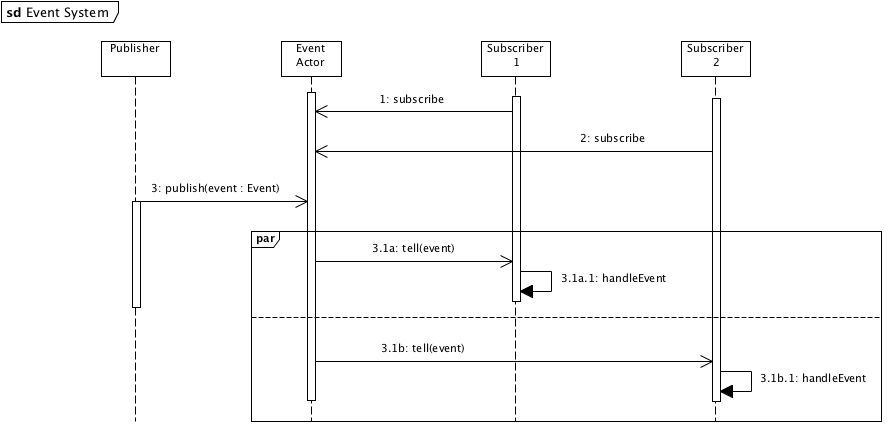
\includegraphics[width=0.8\textwidth]{img/event_system.png}  
   \caption{Funktionsweise des Eventsystems an einem Beispiel}   
  \label{fig:event-system} 
\end{figure}

In Abbildung \ref{fig:event-system} ist der Aufbau des Eventsystems zu sehen. Der Event-Aktor übernimmt die Rolle des Dispatchers und verwaltet die Abonnements. Durch das Starten mehrerer Instanzen des Event-Aktors wird eine Lastverteilung erreicht.

In der Umsetzung erfolgt das Abonnieren einer Nachricht durch das Senden einer partiellen Funktion\footnote{Eine partielle Funktion $f: A \rightarrow B$ ist im Gegensatz zu einer totalen Funktion nicht auf jedem Wert aus $A$ definiert. Für die Anwendung in Scala siehe \cite{partial-function})} an den Dispatcher. Diese Funktion bildet den Typ \tete{Event} auf Unit ab und ist auf allen Events definiert, welche der Subscriber empfangen will. Der Dispatcher benutzt anschließend alle partiellen Funktionen, um eine eingehende Nachricht zu verteilen. Standartmäßig hat ein Subscriber alle Nachrichten abonniert, für die seine \qc{receive}-Funktion definiert ist.

\section{Anbindung der Konnektoren und des Thumbnailgenerators}
